\chapter{AC relations}
As we're dealing with an AC circuit we'll of course use phasors as to make Kirchoffs
laws hold, phasors will be indicated with a hat.
This is going to be quite a long derivation, so buckle up!\\
\section{Derivation of phasor relations}
loop 1 implies
\begin{eqnarray}
	\hat{V}_{AB} - \hat{V}_{CD} &= 0\\
	\hat{V}_{AB} + \frac{i}{\omega C_p} \hat{I}_{CD} &= 0\\
	i \omega C_p\hat{V}_{AB} &= \hat{I}_{CD}
\end{eqnarray}
Loop 2 implies
\begin{eqnarray}
	-\hat{V}_{CD} - 	\frac{i}{\omega C_s} \hat{I}_{CE} + \hat{V}_{AP} &= 0\\
	-\hat{V}_{AB} - 	\frac{i}{\omega C_s}(\hat{I}_{in} - \hat{I}_{CD}) + \hat{V}_{AP}&= 0\\
	-\hat{V}_{AB} - 	\frac{i}{\omega C_s}\left(\frac{\hat{V}_{AB}}{Z_0} - i\omega C_p\hat{V}_{AB}\right) + \hat{V}_{AP}&= 0\\
-\hat{V}_{AB}\left(1 + 	\frac{i}{\omega C_s Z_0} + \frac{C_p}{C_s}\right) + \hat{V}_{AP}&= 0\\
	\hat{V}_{AB}\left(\frac{i}{\omega C_s Z_0} + \frac{C_s + C_p}{C_s}\right) &= \hat{V}_{AP}\\
\end{eqnarray}
So we now have a relation between the phasor of the input power and the one on the parallel part of the antenna:
\begin{equation}
	\boxed{\hat{V}_{AP}=\hat{V}_{AB}\left(\frac{i}{\omega C_s Z_0} + \frac{C_s + C_p}{C_s}\right)} \label{eqn:APphasor}
\end{equation}
Loop 3 implies
\begin{eqnarray}
	\hat{V}_{AS} - \frac{i}{\omega C_a} \hat{I}_{EG} - \hat{V}_{AP} &= 0\\
	\hat{V}_{AS}  - \hat{V}_{AP} &= \frac{i}{\omega C_a} \hat{I}_{EG}\\
	-i\omega C_a\left( \hat{V}_{AS}  - \hat{V}_{AP}\right) &= \hat{I}_{EG}
	\label{eqn:loop3}
\end{eqnarray}
Now if we take a zoomed out look at the circuit we can see another loop: loop 4, the outer part of the circuit.
Note that this carries no additional information as loops 1 + 2 + 3 equal this loop but we'll go through it anyways
as a consistency check:\\
Loop 4 implies:
\begin{eqnarray}
	&\hat{V}_a + \hat{V}_{AS} + \hat{V}_s - \hat{V}_{AB} = 0\\
	&-\frac{i}{\omega C_a}\hat{I}_{GH} + \hat{V}_{AS} - \frac{i}{\omega C_s} \hat{I}_{CE} - \hat{V}_{AB} = 0\\
	&-\frac{i}{\omega C_a}\hat{I}_{EG} + \hat{V}_{AS} - \frac{i}{\omega C_s} \hat{I}_{CE} - \hat{V}_{AB} = 0\\
	&-\left( \hat{V}_{AS}  - \hat{V}_{AP}\right) + \hat{V}_{AS} - \frac{i}{\omega C_s}\left(\frac{\hat{V}_{AB}}{Z_0} + i\omega C_p\hat{V}_{AB}\right) - \hat{V}_{AB} = 0\\
	&\hat{V}_{AP} - \frac{i}{\omega C_s}\left(\frac{\hat{V}_{AB}}{Z_0} + i\omega C_p\hat{V}_{AB}\right) - \hat{V}_{AB} = 0
\end{eqnarray}
Which we have previously encountered, proving that we're consistent.\\
Let's continue on equation \ref{eqn:loop3};
We have that (I couldn't find any relation $f(\hat{V}_{AB}) = \hat{I}_{EG}$):
\begin{equation}
	\hat{I}_{EG} = \frac{\hat{V}_{AS}}{Z_{AS}}
\end{equation}
So
\begin{eqnarray}
	\hat{V}_{AS}\left(1  - \frac{i}{\omega C_a Z_{AS}}\right) &= \hat{V}_{AP}\\
\end{eqnarray}
And using equation \ref{eqn:APphasor} we thus get:
\begin{eqnarray}
	\hat{V}_{AS}\left(1  - \frac{i}{\omega C_a Z_{AS}}\right) &= \hat{V}_{AB}\left(\frac{i}{\omega C_s Z_0} + \frac{C_s + C_p}{C_s}\right)\\
	\hat{V}_{AS} &= \hat{V}_{AB}\frac{\frac{i}{\omega C_s Z_0} + \frac{C_s + C_p}{C_s}}{1  - \frac{i}{\omega C_a Z_{AS}}}\\
\end{eqnarray}
I.e
\begin{equation}
	\hat{V}_{AS} = \hat{V}_{AB}\frac{i C_a Z_{AS} + \omega C_a Z_{AS} Z_0(C_s + C_p)}{\omega C_a C_s Z_{AS} Z_0 - iC_s Z_0}
\end{equation}
Let's split this up into an imaginary and real part:
\begin{eqnarray}
\hat{V}_{AS} &= \hat{V}_{AB}\frac{i C_a Z_{AS} + \omega C_a Z_{AS} Z_0(C_s + C_p)}{\omega C_a C_s Z_{AS} Z_0 - iC_s Z_0}\\
\hat{V}_{AS} &= \hat{V}_{AB}\frac{\left[i C_a Z_{AS} + \omega C_a Z_{AS} Z_0(C_s + C_p)\right](\omega C_a C_s Z_{AS} Z_0 + iC_s Z_0)}{(\omega C_a C_s Z_{AS} Z_0 - iC_s Z_0)(\omega C_a C_s Z_{AS} Z_0 + iC_s Z_0)}\\
\hat{V}_{AS} &= \hat{V}_{AB}\frac{\left[i C_a Z_{AS} + \omega C_a Z_{AS} Z_0(C_s + C_p)\right](\omega C_a C_s Z_{AS} Z_0 + iC_s Z_0)}{(\omega C_a C_s Z_{AS} Z_0)^2 + (C_s Z_0)^2}\\
\hat{V}_{AS} &= \hat{V}_{AB}(C_a C_s Z_{AS} Z_0)\frac{\omega^2 C_a Z_{AS} Z_0(C_s + C_p) - 1 + i\omega  \left[C_a Z_{AS} + Z_0(C_s + C_p)\right]}{(\omega C_a C_s Z_{AS} Z_0)^2 + (C_s Z_0)^2}\\
\hat{V}_{AS} &= \hat{V}_{AB}(C_a Z_{AS} )\frac{\omega^2 C_a Z_{AS} Z_0(C_s + C_p) - 1 + i\omega  \left[C_a Z_{AS} + Z_0(C_s + C_p)\right]}{(\omega C_a^2 C_s Z_{AS}^2 Z_0) + (C_s Z_0)}\\
\hat{V}_{AS} &= \hat{V}_{AB}(C_a Z_{AS})\left[\frac{\omega^2 C_a Z_{AS} Z_0(C_s + C_p)}{(\omega C_a^2 C_s Z_{AS}^2 Z_0) + (C_s Z_0)} + i\frac{\omega  \left[C_a Z_{AS} + Z_0(C_s + C_p)\right]}{(\omega C_a^2 C_s Z_{AS}^2 Z_0) + (C_s Z_0)}\right]\\
\hat{V}_{AS} &= \hat{V}_{AB}\left[\frac{\omega^2 C_a Z_{AS} Z_0(C_s + C_p)}{(\omega C_a C_s Z_{AS} Z_0) + (\frac{C_s Z_0}{C_a Z_{AS}})} + i\frac{\omega  \left[C_a Z_{AS} + Z_0(C_s + C_p)\right]}{(\omega C_a C_s Z_{AS} Z_0) + (\frac{C_s Z_0}{C_a Z_{AS}})}\right]
\end{eqnarray}\\
i.e
\begin{equation}
	\boxed{
	\hat{V}_{AS} = \hat{V}_{AB}\left[\frac{\omega^2 C_a Z_{AS} Z_0(C_s + C_p)}{(\omega C_a C_s Z_{AS} Z_0) + (\frac{C_s Z_0}{C_a Z_{AS}})} + i\frac{\omega  \left[C_a Z_{AS} + Z_0(C_s + C_p)\right]}{(\omega C_a C_s Z_{AS} Z_0) + (\frac{C_s Z_0}{C_a Z_{AS}})}\right]}
\end{equation}
Which is quite a long and difficult equation, we can however make a little approximation, as the capacitors are in the pF range and the frequency is in the MHz range
we have that
\begin{equation}
	\omega C_a C_s Z_{AS} Z_0 \ll \frac{C_s Z_0}{C_a Z_{AS}}
\end{equation}
so
\begin{eqnarray}
	\hat{V}_{AS} &\approx \hat{V}_{AB}\left[\frac{\omega^2 C_a Z_{AS} Z_0(C_s + C_p)}{(\frac{C_s Z_0}{C_a Z_{AS}})} + i\frac{\omega  \left[C_a Z_{AS} + Z_0(C_s + C_p)\right]}{(\frac{C_s Z_0}{C_a Z_{AS}})}\right]\\
	\hat{V}_{AS} &\approx \hat{V}_{AB}\left[\frac{\omega^2 C_a^2 Z_{AS}^2 Z_0(C_s + C_p)}{C_s Z_0} + i\frac{\omega C_a Z_{AS} \left[C_a Z_{AS} + Z_0(C_s + C_p)\right]}{C_s Z_0}\right]\\
	\hat{V}_{AS} &\approx \hat{V}_{AB}\frac{\omega C_a Z_{AS}}{C_s Z_0}\left[\omega C_a Z_{AS} Z_0(C_s + C_p) + i\left[C_a Z_{AS} + Z_0(C_s + C_p)\right]\right]\\
	\hat{V}_{AS} &\approx \hat{V}_{AB}\frac{\omega C_a Z_{AS}}{C_s}\left[\omega C_a Z_{AS} (C_s + C_p) + i\left[C_a \left(\frac{Z_{AS}}{Z_0}\right) + (C_s + C_p)\right]\right]
	\label{eqn:AS_phasor}
\end{eqnarray}
Note that this equation also depends on $Z_{AS}$ which we don't know.
We'll later on see wether we can do something about this.
\newpage
\section{Derivation of measurables}
We'll now convert the phasors to measurables, as
\begin{equation}
	\hat{V}_1 = (a + bi)\hat{V}_2 \implies V_1 = V_0 \sqrt{a^2 + b^2} \cos{(\omega t + \phi)}
\end{equation}
With
\begin{equation}
	\phi = \arctan{\left(\frac{b}{a}\right)}
\end{equation}
From equation \ref{eqn:APphasor}, we have:
\begin{equation}
	V_{AP} = V_0\sqrt{\left(\frac{C_s + C_p}{C_s}\right)^2 + \left(\frac{1}{\omega C_s Z_0}\right)^2}\cos{\left[\omega t + \arctan{\left(\frac{1}{\omega Z_0 (C_S + C_p)}\right)\right]}}
\end{equation}
So resonance over the parallel component of the antenna occurs when 
\begin{equation}
	1 + 2\frac{C_p}{C_s} + \left(\frac{C_p}{C_s}\right)^2 + \frac{1}{(\omega C_s Z_0)^2 }\label{eqn:ResonanceForPar}
\end{equation}
is maximal, in other words, given some angular frequency $\omega$, we may vary $C_p$ and $C_s$ to maximize the power transfer to the parallel component. How this varies
is shown below on a log scale, as can be seen, the ideal position is having $C_s$ as close to 0pF as possible and $C_p$ as close to 1000pF, as is expected when looking
at the circuit. The problem is of course that we don't just need to maximize the power in the parallel system but also in the serial system.
\begin{figure}[ht]
	\centering
	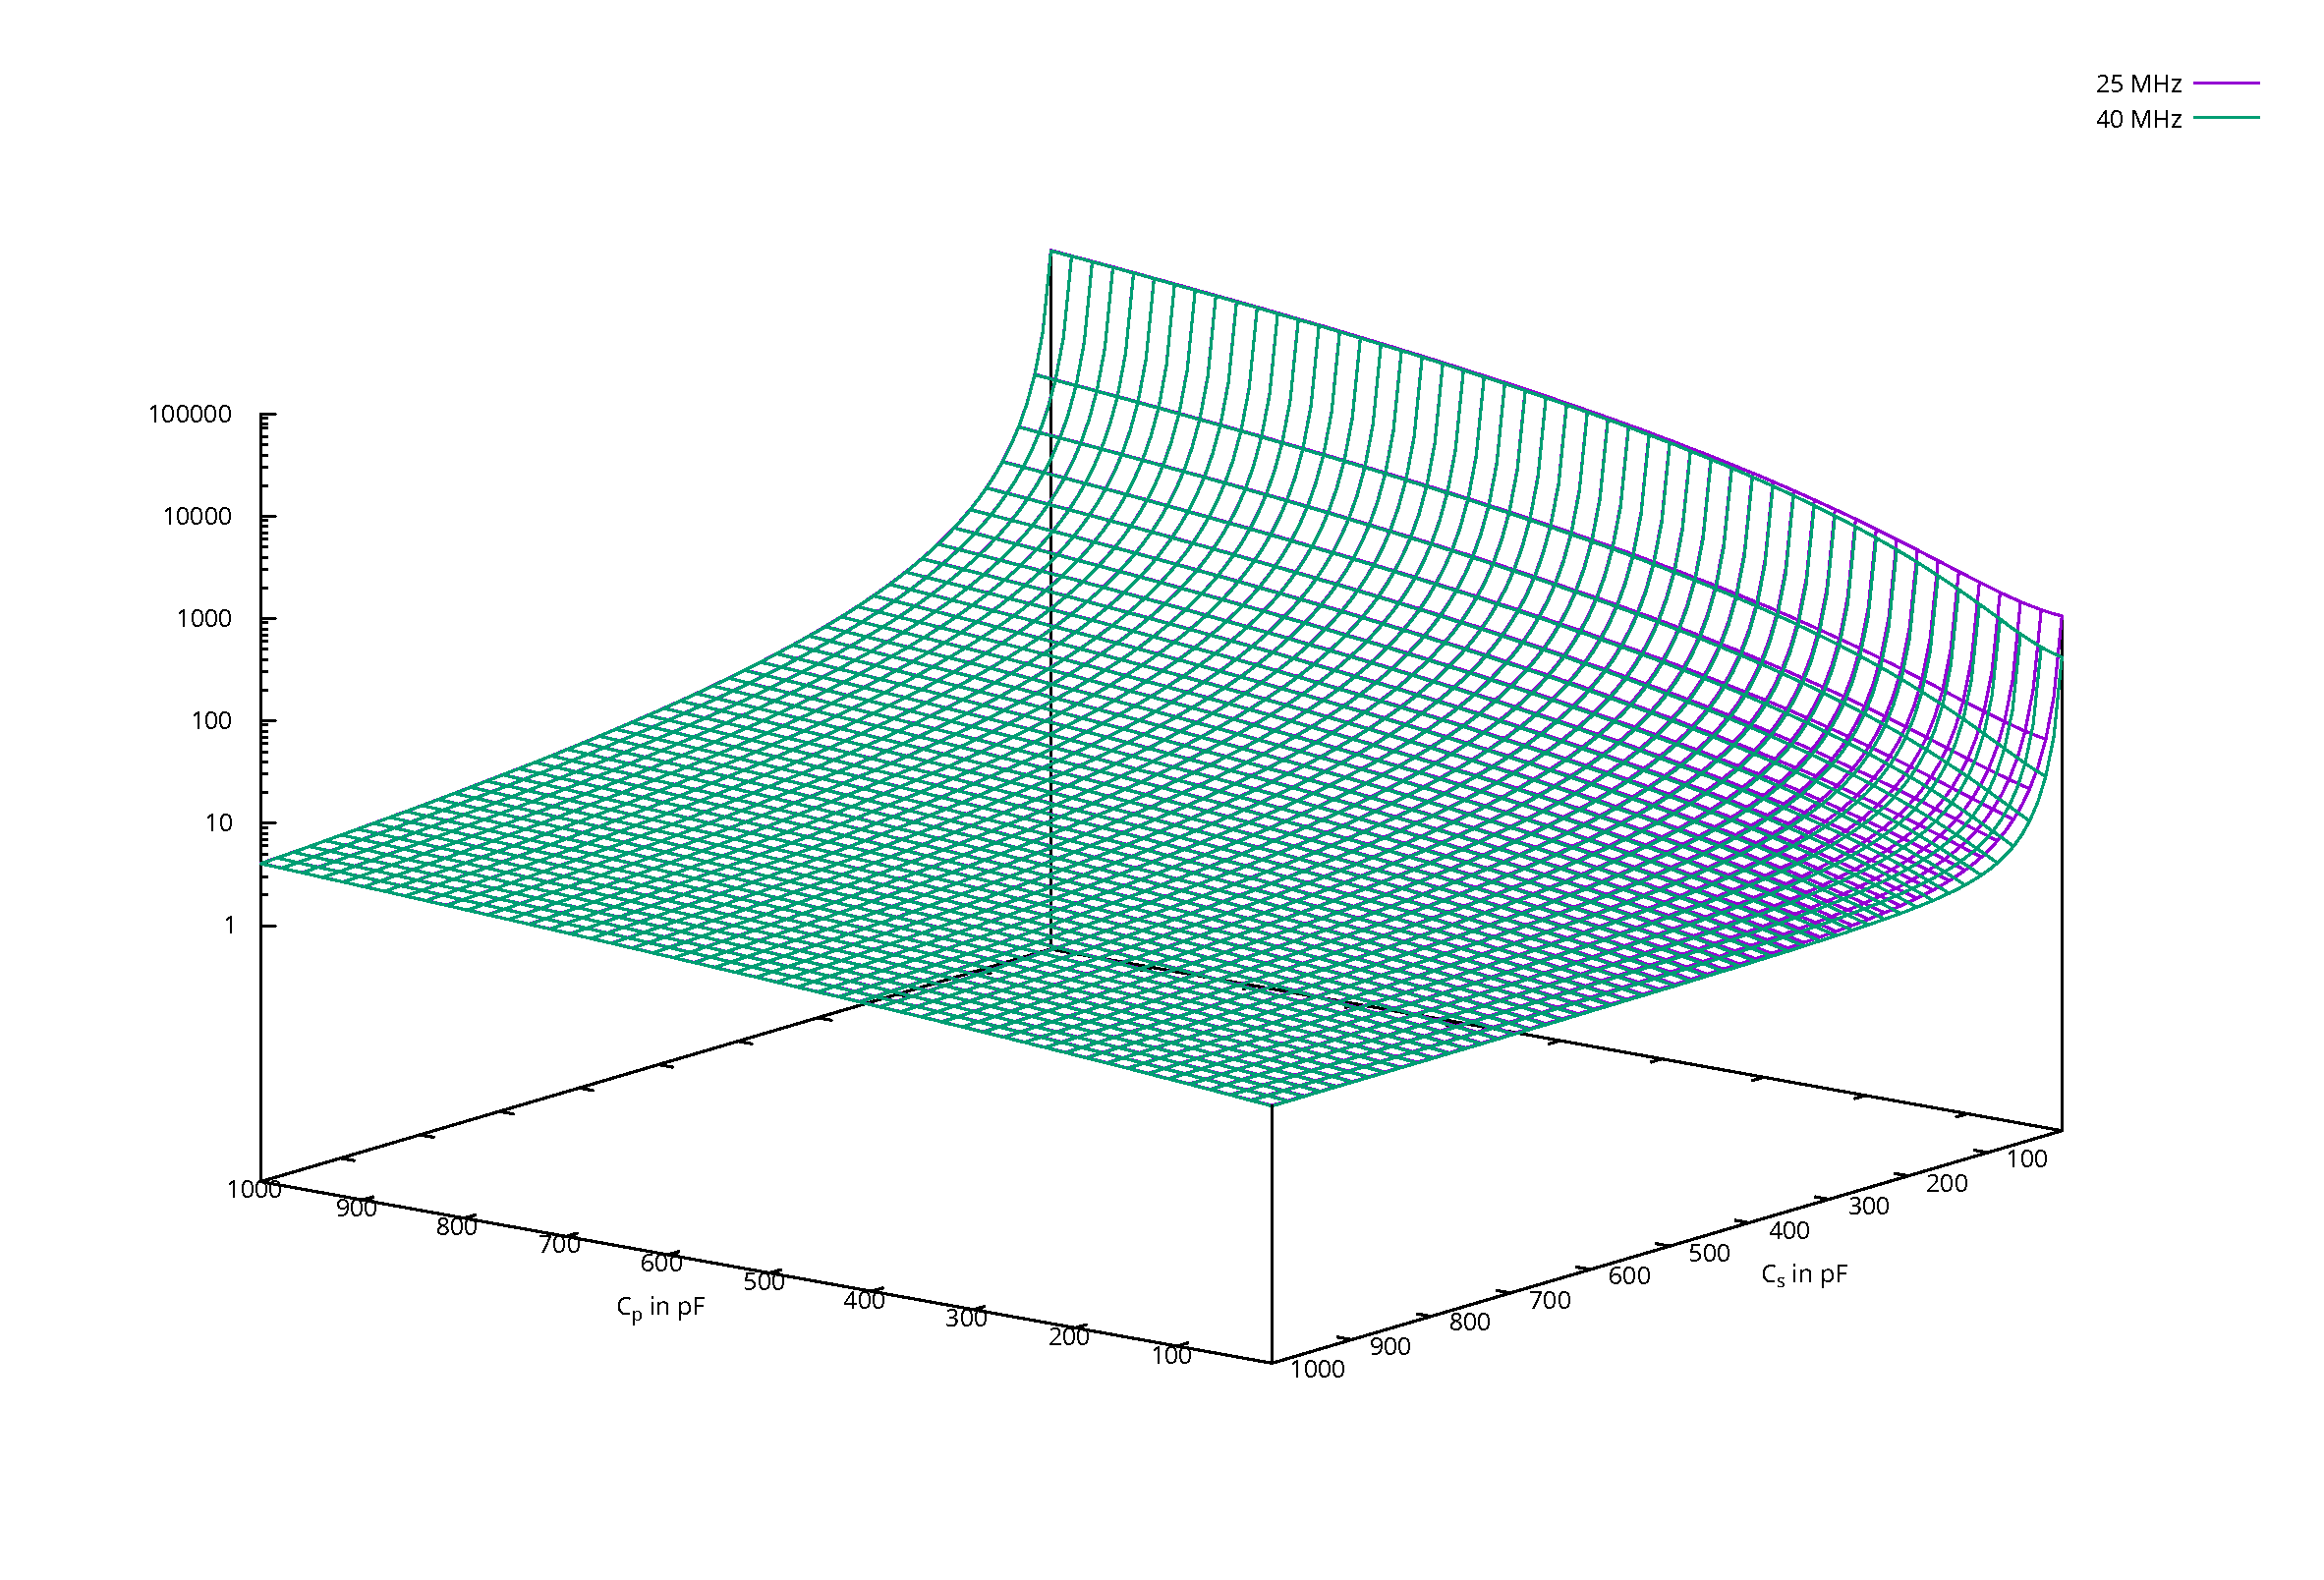
\includegraphics[width=0.9\textwidth]{ParallelMatching.pdf}
\end{figure}\\
From equation \ref{eqn:AS_phasor} we have a phase
\begin{equation}
	\phi = \arctan{\left(\frac{C_a \left(\frac{Z_{AS}}{Z_0}\right) + C_s + C_p}{\omega C_a Z_{AS} (C_s + C_p)}\right)}
\end{equation}
As we somewhat know $\omega$, $C_a$, $C_s$ and $C_p$, by measuring the phase we can thus infer $Z_{AS}$. Now resonance occurs when
\begin{equation}
	\left(\frac{\omega C_a Z_{AS}}{C_s}\right)^2\left[\left(\omega C_a Z_{AS} (C_s + C_p)\right)^2 + \left(C_a \left(\frac{Z_{AS}}{Z_0}\right) + (C_s + C_p)\right)^2\right]
\end{equation}
Is maximal, we'll thus need to maximize the following two equations:\\

\begin{equation}
	\boxed{1 + 2\frac{C_p}{C_s} + \left(\frac{C_p}{C_s}\right)^2 + \frac{1}{(\omega C_s Z_0)^2 }}
\end{equation}
and
\begin{equation}
	\boxed{\left(\frac{\omega C_a Z_{AS}}{C_s}\right)^2\left[\left(\omega C_a Z_{AS} (C_s + C_p)\right)^2 + \left(C_a \left(\frac{Z_{AS}}{Z_0}\right) + (C_s + C_p)\right)^2\right]}
\end{equation}

To obtain resonance over the antenna.
